\documentclass[11pt,preprint, authoryear]{elsarticle}

\usepackage{lmodern}
%%%% My spacing
\usepackage{setspace}
\setstretch{1.2}
\DeclareMathSizes{12}{14}{10}{10}

% Wrap around which gives all figures included the [H] command, or places it "here". This can be tedious to code in Rmarkdown.
\usepackage{float}
\let\origfigure\figure
\let\endorigfigure\endfigure
\renewenvironment{figure}[1][2] {
    \expandafter\origfigure\expandafter[H]
} {
    \endorigfigure
}

\let\origtable\table
\let\endorigtable\endtable
\renewenvironment{table}[1][2] {
    \expandafter\origtable\expandafter[H]
} {
    \endorigtable
}


\usepackage{ifxetex,ifluatex}
\usepackage{fixltx2e} % provides \textsubscript
\ifnum 0\ifxetex 1\fi\ifluatex 1\fi=0 % if pdftex
  \usepackage[T1]{fontenc}
  \usepackage[utf8]{inputenc}
\else % if luatex or xelatex
  \ifxetex
    \usepackage{mathspec}
    \usepackage{xltxtra,xunicode}
  \else
    \usepackage{fontspec}
  \fi
  \defaultfontfeatures{Mapping=tex-text,Scale=MatchLowercase}
  \newcommand{\euro}{€}
\fi

\usepackage{amssymb, amsmath, amsthm, amsfonts}

\def\bibsection{\section*{References}} %%% Make "References" appear before bibliography


\usepackage[round]{natbib}

\usepackage{longtable}
\usepackage[margin=2.3cm,bottom=2cm,top=2.5cm, includefoot]{geometry}
\usepackage{fancyhdr}
\usepackage[bottom, hang, flushmargin]{footmisc}
\usepackage{graphicx}
\numberwithin{equation}{section}
\numberwithin{figure}{section}
\numberwithin{table}{section}
\setlength{\parindent}{0cm}
\setlength{\parskip}{1.3ex plus 0.5ex minus 0.3ex}
\usepackage{textcomp}
\renewcommand{\headrulewidth}{0.2pt}
\renewcommand{\footrulewidth}{0.3pt}

\usepackage{array}
\newcolumntype{x}[1]{>{\centering\arraybackslash\hspace{0pt}}p{#1}}

%%%%  Remove the "preprint submitted to" part. Don't worry about this either, it just looks better without it:
\makeatletter
\def\ps@pprintTitle{%
  \let\@oddhead\@empty
  \let\@evenhead\@empty
  \let\@oddfoot\@empty
  \let\@evenfoot\@oddfoot
}
\makeatother

 \def\tightlist{} % This allows for subbullets!

\usepackage{hyperref}
\hypersetup{breaklinks=true,
            bookmarks=true,
            colorlinks=true,
            citecolor=blue,
            urlcolor=blue,
            linkcolor=blue,
            pdfborder={0 0 0}}


% The following packages allow huxtable to work:
\usepackage{siunitx}
\usepackage{multirow}
\usepackage{hhline}
\usepackage{calc}
\usepackage{tabularx}
\usepackage{booktabs}
\usepackage{caption}


\newenvironment{columns}[1][]{}{}

\newenvironment{column}[1]{\begin{minipage}{#1}\ignorespaces}{%
\end{minipage}
\ifhmode\unskip\fi
\aftergroup\useignorespacesandallpars}

\def\useignorespacesandallpars#1\ignorespaces\fi{%
#1\fi\ignorespacesandallpars}

\makeatletter
\def\ignorespacesandallpars{%
  \@ifnextchar\par
    {\expandafter\ignorespacesandallpars\@gobble}%
    {}%
}
\makeatother

\newlength{\cslhangindent}
\setlength{\cslhangindent}{1.5em}
\newenvironment{CSLReferences}%
  {\setlength{\parindent}{0pt}%
  \everypar{\setlength{\hangindent}{\cslhangindent}}\ignorespaces}%
  {\par}


\urlstyle{same}  % don't use monospace font for urls
\setlength{\parindent}{0pt}
\setlength{\parskip}{6pt plus 2pt minus 1pt}
\setlength{\emergencystretch}{3em}  % prevent overfull lines
\setcounter{secnumdepth}{5}

%%% Use protect on footnotes to avoid problems with footnotes in titles
\let\rmarkdownfootnote\footnote%
\def\footnote{\protect\rmarkdownfootnote}
\IfFileExists{upquote.sty}{\usepackage{upquote}}{}

%%% Include extra packages specified by user
\usepackage{amsmath}

%%% Hard setting column skips for reports - this ensures greater consistency and control over the length settings in the document.
%% page layout
%% paragraphs
\setlength{\baselineskip}{12pt plus 0pt minus 0pt}
\setlength{\parskip}{12pt plus 0pt minus 0pt}
\setlength{\parindent}{0pt plus 0pt minus 0pt}
%% floats
\setlength{\floatsep}{12pt plus 0 pt minus 0pt}
\setlength{\textfloatsep}{20pt plus 0pt minus 0pt}
\setlength{\intextsep}{14pt plus 0pt minus 0pt}
\setlength{\dbltextfloatsep}{20pt plus 0pt minus 0pt}
\setlength{\dblfloatsep}{14pt plus 0pt minus 0pt}
%% maths
\setlength{\abovedisplayskip}{12pt plus 0pt minus 0pt}
\setlength{\belowdisplayskip}{12pt plus 0pt minus 0pt}
%% lists
\setlength{\topsep}{10pt plus 0pt minus 0pt}
\setlength{\partopsep}{3pt plus 0pt minus 0pt}
\setlength{\itemsep}{5pt plus 0pt minus 0pt}
\setlength{\labelsep}{8mm plus 0mm minus 0mm}
\setlength{\parsep}{\the\parskip}
\setlength{\listparindent}{\the\parindent}
%% verbatim
\setlength{\fboxsep}{5pt plus 0pt minus 0pt}



\begin{document}



\begin{frontmatter}  %

\title{The Link Between Market Correlation Structure and the Performance of
Risk-Based Portfolios}

% Set to FALSE if wanting to remove title (for submission)




\author[Add1]{Nathan Potgieter\footnote{\textbf{Contributions:} \newline \emph{The
  author would like to thank Nico Katzke for helping me puzzle and prod
  my to to the eventual completion of this research project.}}}
\ead{19959672@sun.ac.za}





\address[Add1]{Stellenbosch University, Stellenbosch, South Africa}


\begin{abstract}
\small{
This work uses Monte Carlo methods to design and simulate five
distinctive markets types, with each market type possesing a unique
correlation structure in its return matrix. The equal weight, minimum
variance, inverse variance, equal risk contribution and maximum
diversification risk-based portfolios are evaluated in each of the
simulated markets. The relative performance of each portfolio is
compaired within market types and the relationship between portfolio
return characteristics and the market's correlation structure is
investigated \textbf{FINDINGS}
}
\end{abstract}

\vspace{1cm}

\begin{keyword}
\footnotesize{
Monte Carlo \sep Risk-based Portfolios \sep Portfolio Selection
\sep Copula \\ \vspace{0.3cm}
\textit{JEL classification} L250 \sep L100
}
\end{keyword}
\vspace{0.5cm}
\end{frontmatter}



%________________________
% Header and Footers
%%%%%%%%%%%%%%%%%%%%%%%%%%%%%%%%%
\pagestyle{fancy}
\chead{}
\rhead{}
\lfoot{}
\rfoot{\footnotesize Page \thepage}
\lhead{}
%\rfoot{\footnotesize Page \thepage } % "e.g. Page 2"
\cfoot{}

%\setlength\headheight{30pt}
%%%%%%%%%%%%%%%%%%%%%%%%%%%%%%%%%
%________________________

\headsep 35pt % So that header does not go over title




\hypertarget{introduction}{%
\section{\texorpdfstring{Introduction
\label{Introduction}}{Introduction }}\label{introduction}}

Since Markowitz (\protect\hyperlink{ref-markowitz}{1952}) published the
seminal work on mean-variance portfolios, scholars from around the globe
have been striving to develop a robust algorithm capable of situating a
portfolio on the efficient frontier \emph{ex ante}. There are now a wide
array of available portfolio algorithms ranging from simple
heuristic-based approaches to advanced mathematical algorithms based on
quadratic optimization, random matrix theory and machine learning
methods, with many more are still to come.

Unfortunately, the mean-variance portfolios of Markowitz
(\protect\hyperlink{ref-markowitz}{1952}) suffer from sever sensitivity
issues, where slight changes in their expected return input cause large
changes in optimal portfolio weights. This is exacerbated by the fact
that expected returns are notoriously difficult, if not impossible, to
accurately forecast (De Prado, \protect\hyperlink{ref-lopez}{2016}). Due
to this issue, this work focuses solely on so-called risk-based
portfolios, defined by De Carvalho \emph{et al.}
(\protect\hyperlink{ref-leote}{2012}\protect\hyperlink{ref-leote}{a}) as
``systemic quantitative approaches to portfolio allocation'' that solely
rely on views of risk when allocating capital. These strategies do not
require expected return forecasts and, are therefore, said to be more
robust to estimation error. Despite their sole focus on risk mitigation,
empirical back tests have shown that they often perform surprising well,
from a total return standpoint (Choueifaty \emph{et al.},
\protect\hyperlink{ref-choueifaty2013}{2013}).

Rather than using the standard empirical approach to evaluate said
strategies, this work attempts to use Monte Carlo simulation methods.
This allows for an investigation of the link between the markets
covariance structure and portfolio performance. Monte Carlo methods
prove to be invaluable in this investigation. They allow for the
creation of \emph{ad hoc} markets with predetermined risk return
characteristics, and hence leave no uncertainty regarding the
composition of the market. This creates an ideal environment for
experimentation as the researcher has complete control over the market,
and can therefore, adjust the independent variable and observe the
response in the dependent variable. In this study the market correlation
structure serves as the independent variable and the portfolio return
series the dependent variable. Monte Carlo methods are also beneficial
here because they enable the effective reduction of noise in portfolio
performance measures.

The risk-based portfolios evaluated in this work include the naive equal
weight (EW), minimum variance (MV), inverse variance (IV), equal risk
contribution (ERC) and maximum diversification (MD) portfolios. Section
\ref{aims} (below) sets out the aims and objects. Section \ref{lit}
provides a review of the relevant literature; this includes general
issues plaguing the field of portfolio optimization, the rational and
theoretical underpinnings behind the five risk-based portfolios, their
relative performance in empirical back tests and finally, the importance
of using Monte Carlo methods in finance. Section \ref{methadology}
discusses the methodology, Section \ref{reasults} provides and discusses
the results, and Section \ref{conclusion} concludes.

\hypertarget{aims-and-objectives}{%
\section{\texorpdfstring{Aims and Objectives
\label{aims}}{Aims and Objectives }}\label{aims-and-objectives}}

This work aims to use Monte Carlo Methods to uncover the relationship
between a market's correlation structure and the risk return properties
of various risk-based portfolio algorithms. This is achieved through the
following objectives:

\begin{enumerate}
\def\labelenumi{\arabic{enumi}.}
\item
  Design and create four distinctive \emph{ad hoc} correlation matrices
  and estimate one empirical correlation matrix, each describing a
  market of 50 assets with a unique correlation structure. These
  matrices range from those possessing no clusters, to those exhibiting
  hierarchical clustering.
\item
  Use these five correlation matrices as the key input in their own
  Monte Carlo simulation, where each correlation matrix corresponds to a
  unique market type. All other risk characteristics remain equal
  between market types. The markets will each be built with a student t
  multivariate distribution with 4.5 degrees of freedom. The individual
  asset's univariate distributions will each be normally distributed
  with means and standard deviations calibrated with S\&P500 data. Each
  of the five market types will be simulated 10 000 times across 500
  periods, or approximately two years of trading daily return data.
\item
  Calculate the returns obtained from each risk-based portfolio in each
  of the simulated markets. Use the first 250 periods to estimate an out
  of sample covariance matrix and calculate portfolio weights. Conduct
  periodic rebalancing every 50 periods, each time looking back 250
  periods, recalculating the covariance matrix and the new portfolio
  weights. Repeat this process until all 500 simulated periods have been
  considered.
\item
  Calculate the average Sharp ratio, standard deviation, downside
  deviation, value at risk (VaR), effective number of constitutes (ENC)
  and effective number of bets (ENB) for each portfolio across the 10
  000 markets for each market type.
\item
  Compare the relative performance of each portfolio within each of the
  market types and evaluate how the relative performance of each
  portfolio is effected by the change in market correlation structure.
\end{enumerate}

\hypertarget{litrature-review}{%
\section{\texorpdfstring{Litrature Review
\label{lit}}{Litrature Review }}\label{litrature-review}}

\hypertarget{review-of-portfolio-optimisation-algorithms}{%
\subsection{Review of Portfolio Optimisation
Algorithms}\label{review-of-portfolio-optimisation-algorithms}}

\hypertarget{introduction-1}{%
\subsubsection{Introduction}\label{introduction-1}}

This literature review will cover common issues reported in the
literature of portfolio optimization, the five risk-based portfolios
evaluated in this work, their respective performance in both empirical
back tests and Monte Carlo studies and finally the importance of using
Monte Carlo methods within the field of finance.

\hypertarget{issues-with-portfolio-optimization}{%
\subsubsection{Issues with Portfolio
optimization}\label{issues-with-portfolio-optimization}}

When operating in sample, portfolio optimization tends to be a perfect
science, out of sample it becomes more of an art form where it is often
preferable to use simple heuristic over advanced techniques. This
section highlights some general issues that tend to worsen their
performance out of sample.

Firstly, mean-variance optimizers, like those introduced by Markowitz
(\protect\hyperlink{ref-markowitz}{1952}), rely heavily on the accuracy
of their expected return forecasts. Small changes in their expected
return input can lead to large changes in portfolio weights (De Prado,
\protect\hyperlink{ref-lopez}{2016}). Since, in practice, expected
returns are extremely difficult to estimate accurately, this issue
serves as a hindrance to their wide spread use. Therefore, the so-called
risk based portfolios that intentionally avoid using expected return
forecasts have garnered a lot of attention (Maillard,
\protect\hyperlink{ref-maillard2010}{2010}).

However, these risk-based portfolios are not void of issues. The
quadratic programming methods used in many portfolio optimizers,
including Markovitz's (1952) mean-variance and some risk-based
portfolios, require the inversion of some positive-definite covariance
matrix. This requirement for positive definiteness can cause issues, as
covariance matrices estimated on empirical data are sometimes not
positive definite, in which case their inverse does not exist and these
portfolios do not have solutions (De Prado,
\protect\hyperlink{ref-lopez}{2016}). One approach that alleviates this
issue is to simply compute the nearest positive definite matrix and use
that instead (Bates \& Maechler, \protect\hyperlink{ref-Matrix}{2019};
Higham, \protect\hyperlink{ref-higham2002}{2002}).

The covariance matrix estimation step is susceptible to measurement
error, particularly if the underlying covariance matrix suffers from a
high condition number (Zhou \emph{et al.},
\protect\hyperlink{ref-zhou2019}{2019}). A condition number is defined
as the absolute value of the ratio between a covariance matrix's largest
and smallest eigenvalues (Bailey \& Lopez De Prado,
\protect\hyperlink{ref-lopez2012}{2012}; De Prado,
\protect\hyperlink{ref-lopez}{2016}). The condition number is smallest
in diagonal matrices (equal to 1) and increases as more correlated
variables are added. When working with high condition number matrices, a
small change in a single entry's estimated covariance can greatly alter
its inverse, which in turn can effect the portfolio weights (De Prado,
\protect\hyperlink{ref-lopez}{2016}). This is related to Markowitz's
curse which De Prado (\protect\hyperlink{ref-lopez}{2016}) summarized by
stating that ``the more correlated investments are, the greater is the
need for a diversified portfolio---and yet the greater are that
portfolio's estimation errors''.

For a sample with a given number of periods, larger dimension covariance
matrices are prone to more noise in estimation. This is essentially due
to a reduction in degrees of freedom as a sample of at least
\(1/2N(N+1)\) independent and identically distributed (iid) observations
is required to estimate an \(N\times N\) covariance matrix (De Prado,
\protect\hyperlink{ref-lopez}{2016}: 60){]}. Furthermore, financial
market covariance structures tend to vary over time and have been known
to change rapidly during so-called regime changes (De Prado,
\protect\hyperlink{ref-lopez}{2016}). This exacerbates the issue of
requiring a large number of observations when estimating the covariance
matrix, since passed data may not be a good refection of the future and
looking further increases this likelihood.

\hypertarget{risk-based-portfolios}{%
\subsubsection{Risk Based Portfolios}\label{risk-based-portfolios}}

This section reviews the intuition and technical underpinnings within
the literature on risk-based portfolios. Those discussed here include
the equal weight (EW), minimum variance (MV), inverse volatility (IV),
equal risk contribution (ERC) and maximum diversification (MD)
portfolios. The EW is a simple heuristic approach, the minimum variance
is more akin to a Markowitz (\protect\hyperlink{ref-markowitz}{1952})
mean-variance portfolio, while the inverse-variance (IV), equal risk
contrition (ERC) and maximum diversification (MD) are quite similar in
that they all assume that adequate diversification can be obtained by
allocating equal risk to each investible security.

\hypertarget{naive-equal-weight-ew}{%
\paragraph{Naive Equal Weight (EW)}\label{naive-equal-weight-ew}}

Perhaps the oldest and most simple approach to portfolio diversification
involves holding a weight of \(1/N\) of the \(N\) total available assets
(DeMiguel \emph{et al.}, \protect\hyperlink{ref-demiguel2009}{2009}). In
other words, this strategy can be described as putting an equal number
of eggs into each available basket. It does not require any historical
data when allocating capital and does not involve any form of
optimization (DeMiguel \emph{et al.},
\protect\hyperlink{ref-demiguel2009}{2009}). This portfolio is commonly
called the `equal weight' or 1/N portfolio, however, its failure to
recognize the importance of both asset variance and the covariance
between assets has resulted in it also being referred to as the `naive
portfolio'. Meanwhile, its simplicity means that it has been widely used
as a benchmark. Equal weighting is optimal from a mean-variance
standpoint when there is no correlation between securities, and each
possesses the same variance. In which case, the EW is theoretically
equivalent to the MV portfolio. The EW's robustness to estimation errors
and surprisingly good historical performance has lead to it being
incorporated into hybrid portfolio strategies (Tu \& Zhou,
\protect\hyperlink{ref-tu2011}{2011}). These strategies form a balance
between the rules based approach of the EW and the optimization
approaches from more sophisticated portfolios and have been shown to
outperform both its EW and more sophisticated constituents.

\hypertarget{minimum-variance-mv}{%
\paragraph{Minimum Variance (MV)}\label{minimum-variance-mv}}

Portfolio optimizers designed to exhibit the minimum variance have over
the years garnered a lot of attention. This can in large part be
attributed to their tendency to achieve surprisingly high returns and
low variance in some historical back tests (Clarke \emph{et al.},
\protect\hyperlink{ref-clarke2011}{2011}). Their excellent performance
has been attributed to the empirical phenomena that low volatility
stocks tend to earn returns in excess of the market, and high beta
stocks tend not to be rewarded by higher returns (Clarke \emph{et al.},
\protect\hyperlink{ref-clarke2011}{2011}; Fama \& French,
\protect\hyperlink{ref-fama1992}{1992}). Interesting, this latter
finding contradicts traditional financial economic theory which predicts
an asset's expected return to be proportional to its market beta
(i.e.~undiversifiable risk) (Perold,
\protect\hyperlink{ref-perold2004}{2004}).

The minimum variance portfolio selects security weights such that the
resulting portfolio corresponds to that with the lowest possible in
sample volatility. Therefore, it has the lowest expected volatility and
is, in theory, the safest and least risky portfolio (De Carvalho
\emph{et al.},
\protect\hyperlink{ref-rawl2012}{2012}\protect\hyperlink{ref-rawl2012}{b}).
Its primary input is a variance covariance matrix, which it uses to
minimize aggregate portfolio volatility. This is accomplished by
over-weighting low volatility and low correlation securities (De
Carvalho \emph{et al.},
\protect\hyperlink{ref-rawl2012}{2012}\protect\hyperlink{ref-rawl2012}{b}).
Interestingly, it is the only portfolio of the efficient frontier that
does not depend on expected return forecasts (De Prado,
\protect\hyperlink{ref-lopez}{2016}).

The following provides a technical explanation of how the MV portfolio's
weights are calculated. Let \(\sum\) indicate the markets variance
covariance matrix and \(w=\{w_i,..., w_N \}\) be a vector of length N
containing individual security weights. The vector containing the MV
portfolio's weights can now be described as (De Carvalho \emph{et al.},
\protect\hyperlink{ref-rawl2012}{2012}\protect\hyperlink{ref-rawl2012}{b}):

\begin{center}
$w^*=arg\min(w'\sum w)\ \ \ s.t.\ \sum^N_iw_i=1$ 
\end{center}

In some studies, the minimum variance (MV) portfolio has been found by
to earn cumulative returns equal to or slightly greater than market
capitalization weighted portfolio's, whilst maintaining a consistently
lower variance and achieving a noticeable improvement in downside risk
mitigation (Clarke \emph{et al.},
\protect\hyperlink{ref-clarke2011}{2011}). The MV portfolio can,
therefore, work well out of sample, but if left unrestricted, tends to
concentrate its holdings in a small number of assets (De Prado,
\protect\hyperlink{ref-lopez}{2016}). Its sole objective to minimize
portfolio volatility is likely the the primary reason for this. When
near the trough of its objective function, it to achieves minor
reductions in \emph{ex ante} volatility by greatly favoring a small
number of low volatility/correlation securities (De Prado,
\protect\hyperlink{ref-lopez}{2016}: 68){]}. This tendency to produce
highly concentrated portfolio's can be costly out of sample since the
portfolio exposed to the idiosyncratic risk of its major constituents.
It puts too many eggs in too few baskets. In practice, this issue can be
countered by applying cleaver maximum and minimum portfolio weight
constraints.

\hypertarget{inverse-varience-iv-weighting}{%
\paragraph{Inverse-Varience (IV)
Weighting}\label{inverse-varience-iv-weighting}}

The IV portfolio, referred to as the equal-risk budget (ERB) portfolio
in De Carvalho \emph{et al.}
(\protect\hyperlink{ref-leote}{2012}\protect\hyperlink{ref-leote}{a}),
aims to allocate an equal risk budget to each investible security. Where
the risk budget is defined as the the product of a security's weight and
volatility (De Carvalho \emph{et al.},
\protect\hyperlink{ref-leote}{2012}\protect\hyperlink{ref-leote}{a}). If
\(\sigma_i\) is defined as security i's volatility, then the portfolio
risk budget can be equally distributed across N securities by setting
security weights as:

\begin{center} 
$w_{iv}=(\frac{1/\sigma_1}{\sum^N_{j=1} 1/\sigma}, ...,\frac{1/\sigma_N}{\sum^N_{j=1} 1/\sigma} )$ 
\end{center}

This indicates that each securities weight is directly proportional to
the inverse of its variance, thereby demonstrating why this is called
the IV portfolio. The IV portfolio allocates capital based solely on
security variance and, is therefore, oblivious to the covariance between
its constitutes. De Carvalho \emph{et al.}
(\protect\hyperlink{ref-leote}{2012}\protect\hyperlink{ref-leote}{a})
found that, if all securities posses the same sharp ratio and their
correlation coefficients are all equal, then the IV portfolio is
efficient from a mean-variance stand point and obtains the highest
possible sharp ratio.

\hypertarget{equal-risk-contribution-erc}{%
\paragraph{Equal Risk Contribution
(ERC)}\label{equal-risk-contribution-erc}}

The principle behind the ERC portfolio is similar to that of the IV,
however, when balancing risk contributions the ERC does account for the
covariance between securities (De Carvalho \emph{et al.},
\protect\hyperlink{ref-leote}{2012}\protect\hyperlink{ref-leote}{a}).
The ERC allocates capital such that each security contributes equally to
overall portfolio risk, which in theory should maximize risk
diversification (Maillard, \protect\hyperlink{ref-maillard2010}{2010}).
According to Maillard (\protect\hyperlink{ref-maillard2010}{2010}), in
practice the ERC acts similar to a weight constrained MV portfolio, with
constraints preventing high levels of portfolio concentration. Following
the derivation and notation of Maillard
(\protect\hyperlink{ref-maillard2010}{2010}), the weights of an ERC
portfolio \(x=(x_1,x_2,...,x_n)\) consisting of n assets can be
calculated as follows:

Let \(\sigma_i^2\) resemble asset i's variance, \(\sigma_{ij}\) the
covariance between asset i and j and \(\sum\) be the markets variance
covariance matrix. Portfolio risk can now be written as
\(\sigma(x)=\sqrt{x^T\sum x}=\sum_i\sum_{j\neq i}x_ix_j\sigma_{ij}\) and
the marginal risk contribution, \(\partial_{x_i}\sigma(x)\), can then be
defined as:

\begin{center}
$\partial_{x_i}\sigma(x)=\frac{\partial\sigma(x)}{\partial x_i}=\frac{x_i\sigma_i^2+\sum_{j\neq i}x_j\sigma_{ij}}{\sigma(x)}$ 
\end{center}

Therefore, \(\partial_{x_i}\sigma(x)\) refers to the change in portfolio
volatility resulting from a small change in asset i's weight (Maillard,
\protect\hyperlink{ref-maillard2010}{2010}). ERC uses this definition to
guide central objective to equate the risk contribution across each of
the n assets. There is no closed-form solution describing the weights of
the ERC portfolio, however, if we define \((\sum x)_i\) as the
\(i^{th}\) row resulting from the product of \(\sum\) with x and note
that \(\partial_{x_i}\sigma(x)=(\sum x)_i\), then optimal security
weights, for the long only ERC portfolio, can be described as those that
satisfy the following statement (see Maillard
(\protect\hyperlink{ref-maillard2010}{2010}), p.~4-7 for more detail):

\begin{center}
$x^*=\{x \ \epsilon[0,1]^n:\sum x_i=1, x_i \times (\sum x)_i=x_j \times (\sum x)_j \ \forall  \ i,j \}$ 
\end{center}

Maillard (\protect\hyperlink{ref-maillard2010}{2010}) proved
mathematically that the ERC portfolio's \emph{ex ante} volatility is
always somewhere between those of the EW and MV portfolios. De Carvalho
\emph{et al.}
(\protect\hyperlink{ref-leote}{2012}\protect\hyperlink{ref-leote}{a})
found that, if all securities posses the same sharp ratio, then the ERC
and IV portfolios have identical weights. If, in addition, the
correlation coefficients between all securities are equal, then the ERC
and IV merge into the EW portfolio, with each being mean variance
efficient with the maximum attainable sharp ratio (De Carvalho \emph{et
al.},
\protect\hyperlink{ref-leote}{2012}\protect\hyperlink{ref-leote}{a}).

\hypertarget{maximum-diversification-md}{%
\paragraph{Maximum Diversification
(MD)}\label{maximum-diversification-md}}

Choueifaty \& Coignard (\protect\hyperlink{ref-choueifaty2008}{2008})
originally designed the MD portfolio to maximize some diversification
ratio (DR), which he defined as the sum of each securities risk bucket
(\(w'.V\)) divided by portfolio volatility (De Carvalho \emph{et al.},
\protect\hyperlink{ref-leote}{2012}\protect\hyperlink{ref-leote}{a}). If
we define V as a vector of asset volatilities and \(\sum\) as the
covariance matrix and \(w^*\) as the vector of MD portfolio weights.
Then the the \(w*\) can be expressed as:

\begin{center} 
$w^* =arg\ max(DR)\ \ \ \ with \ \ \ \  DR= \frac{w'.V}{\sqrt{w'Vw}}$ 
\end{center}

De Carvalho \emph{et al.}
(\protect\hyperlink{ref-leote}{2012}\protect\hyperlink{ref-leote}{a})
found that, in practice, the MV achieves a diversification ratio similar
to that of the MD, and that the difference between the two is due to the
MV's larger exposure to low residual volatility securities. Much like
the IV and ERC portfolios, the MD portfolio attempts to diversify its
portfolio by allocating equal risk to each security (Choueifaty \&
Coignard, \protect\hyperlink{ref-choueifaty2008}{2008}). The MD
portfolio accomplishes this by over-weighting low volatility and low
correlation securities (De Carvalho \emph{et al.},
\protect\hyperlink{ref-leote}{2012}\protect\hyperlink{ref-leote}{a}).
For further detail regarding the theoretical results and properties of
the MD portfolio see Choueifaty \& Coignard
(\protect\hyperlink{ref-choueifaty2008}{2008}: 33--35).

\hypertarget{empirical-backtests-and-monte-carlo-findings}{%
\subsection{Empirical Backtests and Monte Carlo
Findings}\label{empirical-backtests-and-monte-carlo-findings}}

Choueifaty \emph{et al.} (\protect\hyperlink{ref-choueifaty2013}{2013})
used empirical back testing to compare the relative performance of
numerous portfolio optimisers. They used historical data from the MSCI
world index and considered the largest 50\% of assets at each
semi-annual rebalance date between 1999 and 2010. To reduce the noise in
estimation, at each rebalance date, covariance matrices were estimated
using the previous years worth of data (Choueifaty \emph{et al.},
\protect\hyperlink{ref-choueifaty2013}{2013}). These were then used as
the primary inputs in estimating the long-only portfolio weights. The MV
portfolio achieved an annual return of 6.7\% and outperformed the ERC
and EW portfolios which returned 6.3\% and 5.8\% respectively. The MV
portfolio achieved the lowest daily volatility (10\%) followed by the
ERC and then the EW portfolio's (with 12.9\% and 16.4\% respectively).
Accordingly, the MV portfolio had the highest sharp ratio (0.36)
followed by the ERC and EW portfolios (0.24 and 0.16, respectively).

Despite the simplistic nature of the EW portfolio, empirical studies
comparing it to the mean-variance, MV and Bayes-Stein portfolios often
report statistically insignificant differences in Sharp ratio between
the EW more the advanced portfolios (DeMiguel \emph{et al.},
\protect\hyperlink{ref-demiguel2009}{2009}). In addition, the EW
performed surprisingly well from a total return perspective. In fact,
many studies have found that the EW portfolio outperforms the mean
variance and other sophisticated portfolios that are based on financial
theory (Tu \& Zhou, \protect\hyperlink{ref-tu2011}{2011}).

Due to the aforementioned issues surrounding covariance matrix
estimation error, Ardia \emph{et al.}
(\protect\hyperlink{ref-ardia2017}{2017}) set out to evaluate the impact
of covariance matrix misspecification on the properties of risk-based
portfolio's. The authors used Monte Carlo methods to build six
distinctive investment universes, each with a unique covariance
structure. Numerous covariance matrix estimation techniques were then
used on the simulated data, one of which served as the benchmark. They
then accessed the impact of alternative covariance specifications on the
performance of the MV, IV, ERC and MD portfolio's. The ERC and IV
portfolios were found to be ``relatively robust to covariance
misspecification'', the MV was found to be sensitive to misspecification
in both the variance and covariance and the MD portfolio was found to be
robust to variances misspecification but sensitive to misspecification
in the covariances (Ardia \emph{et al.},
\protect\hyperlink{ref-ardia2017}{2017}: 1).

\hypertarget{monte-carlo-methods-in-portfolio-optimisation}{%
\subsection{Monte Carlo Methods in Portfolio
Optimisation}\label{monte-carlo-methods-in-portfolio-optimisation}}

Ever since the pioneering age of computers people have shown a keen
interest in leveraging their ability to perform rapid calculations to
conduct randomized experiments. The core of Monte Carlo simulation is in
the creation of random objects and/or processes using a computer (Kroese
\emph{et al.}, \protect\hyperlink{ref-kroese2014}{2014}: 1). There are a
number of reasons for doing this, but the primary one used in this work,
and thereby discussed in this review, is of the sampling kind (Kroese
\emph{et al.}, \protect\hyperlink{ref-kroese2014}{2014}). This typically
involves the modeling of some stochastic object or process, followed by
sampling from some probability distribution and the manipulating said
sample through some deterministic process such that the result mimics
the true underlying process. The primary idea behind Monte Carlo
simulation is to repeat this simulation process many times so that
interesting properties can be uncovered through the law of large numbers
and central limit theorem (Glasserman,
\protect\hyperlink{ref-glasserman2013}{2013}).

A financial application of this can be found in Wang \emph{et al.}
(\protect\hyperlink{ref-wang2012}{2012}) who designed a Monte Carlo
procedure that (1) models both the time-series and cross-section
properties of financial market returns, involving the use of extreme
value theory to estimates a random term's probability distribution
function (pdf), and (2) sampling from the modeled process to produce an
ensemble of market returns, with each exerting the same risk properties.
The simulated data can then be used in risk management and/or the
pricing of financial securities (Kroese \emph{et al.},
\protect\hyperlink{ref-kroese2014}{2014}; Wang \emph{et al.},
\protect\hyperlink{ref-wang2012}{2012}). This unique ability to generate
a large number of counterfactuals for an asset market with a known risk
structure has made it a uniquely powerful tool in accessing the
properties of portfolio optimization algorithms (Bailey \& Lopez De
Prado, \protect\hyperlink{ref-lopez2012}{2012}). See Glasserman
(\protect\hyperlink{ref-glasserman2013}{2013}) as a useful source for
understanding the methods and applications of Monte Carlo methods in
finance.

\hypertarget{methadology}{%
\section{\texorpdfstring{Methadology
\label{methadology}}{Methadology }}\label{methadology}}

This work used Monte Carlo simulation methods to investigate the link
between a markets correlation structure and the relative performance of
the EW, MV, IV, ERC and MD portfolios.

\begin{itemize}
\tightlist
\item
  The term market refers to a set of daily returns for a number of
  assets. For example the daily returns for each of the JSE ALSI
  constitutes between 1 January 2019 and 1 January 2020. Since this is a
  Monte Carlo study, thousands of markets are simulated, they can
  therefore, be thought of as a single observation from a population of
  markets.
\item
  The term `market type' refers to a population of markets each with the
  same specified risk characteristics.
\end{itemize}

The R package MCmarket was used to simulate 10 000 markets from five
separate market types, with the correlation structure being the only
differentiating factor between between market types. (Potgieter,
\protect\hyperlink{ref-MCmarket}{2020}). Four of the correlation
structures/matrices were designed \emph{ad hoc}, while the fifth was
estimated using S\&P 500 data. These correlation matrices range from one
exhibiting no correlation (i.e.~a diagonal matrix) to one with a
hierarchical clustering structure (see Section \ref{corr_struc}).

Thereafter, the long only EW, MV, IV, ERC and MD portfolios were back
tested on the simulated markets (Section \ref{backtest}) and portfolio
analytics were calculated and aggregated across the 10 000 markets
(Section \ref{portmet}). Finally, the portfolio metrics are compared
within market types across portfolios and within portfolios, across
market types.

\hypertarget{correlation-structures}{%
\subsection{\texorpdfstring{Correlation Structures
\label{corr_struc}}{Correlation Structures }}\label{correlation-structures}}

This section discusses the five correlation matrices used in the Monte
Carlo simulations. Section \ref{adhoc} describes the composition and
attributes of the four \emph{ad hoc} correlation matrices. While Section
\ref{emp} describes the methodology behind the estimation of the
empirical correlation matrix. Each of the five matrices top 10
eigenvalues are listed in Table \ref{eigens}.

\hypertarget{ad-hoc}{%
\subsubsection{\texorpdfstring{Ad Hoc
\label{adhoc}}{Ad Hoc }}\label{ad-hoc}}

This section describes the four \emph{ad hoc} 50 by 50 correlation
matrices used as the key inputs in their respective Monte Carlo
simulations. See Figure \ref{corr_mats} for a graphical representation
of each correlation matrix. Note that the \emph{gen\_corr} function from
the R package \emph{MCmarket} was used in the construction of the four
\emph{ad hoc} matrices (Potgieter,
\protect\hyperlink{ref-MCmarket}{2020}).

The first and most simplistic of the four matrices is a diagonal matrix
(see Diagonal Matrix in Figure \ref{corr_mats}). It describes a market
with a zero correlation coefficient between each asset. Each of its 50
eigenvalues are equal to 1 (Table \ref{eigens}), it has no risk clusters
and has plenty scope for diversification. This correlation matrix has
the lowest possible condition number of 1. The Monte Carlo data set
constructed using this matrix is referred to as Market 1.

The second matrix (labeled No Clusters in Figure \ref{corr_mats}) has no
risk clusters but describes a market with significant correlation
between its constituents. Each asset has a correlation of 0.9 with its
closest neighbor (i.e.~Asset 1 and 2, 5 and 6 and 11 and 12 each have a
pairwise correlation coefficient of 0.9). Correlations then diminish
exponentially by the absolute distance between the two assets (i.e.~the
correlation between Asset 1 and 5 is \(0.9^{|1-5|}=0.6561\)). It has a
large first eigenvalue of 15.93, but they quickly diminish in size, such
that, its 9th largest eigenvalue is less than 1 at 0.79 (Table
\ref{eigens}). This correlation matrix has the highest condition number
of 302.4. The Monte Carlo data set constructed using this matrix is
referred to as Market 2.

The third matrix (labeled Five Clusters in Figure \ref{corr_mats})
contains five distinct non-overlapping risk clusters. Assets within the
same cluster have a pairwise correlation coefficient of 0.6 while those
that are not in the same cluster are uncorrelated. This correlation
matrix has a condition number of 16.1. The Monte Carlo data set
constructed using this matrix is referred to as Market 3.

The final \emph{ad hoc} correlation matrix has three layers of
overlapping risk clusters. The first layer has 10 distinctive clusters,
within which, assets have a correlation coefficient of 0.7. The second
layer has four clusters where assets that are not in same first layer
cluster have a correlation coefficient of 0.5. Assets that are in the
same third layer cluster but not clustered in layers one and two have a
correlation coefficient of 0.3. Finally, those that do not share any
cluster have a correlation coefficient of 0.05. Its largest eigenvalue
is 14.36, but they diminish fairly quickly as its third largest is only
3.3 (Table \ref{eigens}). This correlation matrix has a condition number
of 47.9. The Monte Carlo data set constructed using this matrix is
referred to as Market 4.

\begin{figure}
\centering
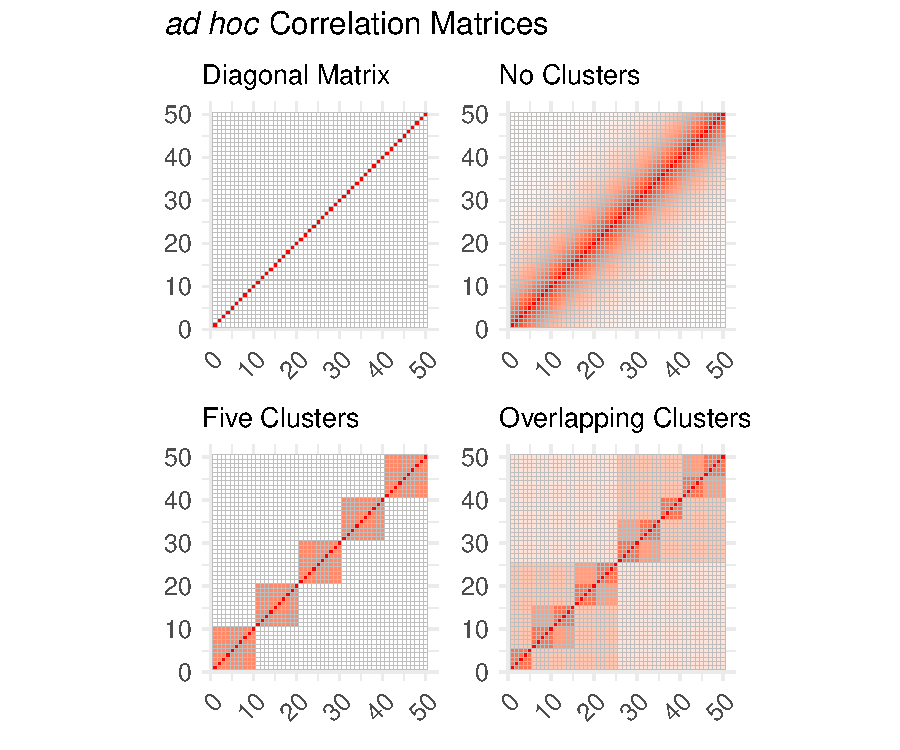
\includegraphics{Thesis_files/figure-latex/corr mats-1.pdf}
\caption{\label{corr_mats} Correlation Matrices}
\end{figure}

\hypertarget{emperical}{%
\subsubsection{\texorpdfstring{Emperical
\label{emp}}{Emperical }}\label{emperical}}

The empirical correlation matrix used in this study was estimated from
the daily returns of a random subset of 50 of the largest 100 S\&P 500
stocks, determined by market capitalization, between 1 January 2016 and
1 January 2021. The market capitalizations were measured as of 12
January 2020.

The markets covariance matrix was then estimated using the
\emph{fit\_mvt} function from the R package \emph{fitHeavyTail} (Palomar
\& ZHOU, \protect\hyperlink{ref-fitHeavyTail}{2020}). This covariance
estimation method uses maximum likelihood estimation and generalized
expectation maximization to fit a multivariate t-distribution to a
matrix of asset returns (Liu \& Rubin,
\protect\hyperlink{ref-liu1995}{1995}). The estimated multivariate t
distribution was found to have 4.43 degrees of freedom and a correlation
matrix shown in Figure \ref{corr_emp}.

Note that in Figure \ref{corr_emp} assets were ordered by hierarchical
clustering so that the reader could more easily visualize the risk
clusters. The correlation matrix's largest eigenvalue is 18.6 and they
quickly diminish to below zero by its 8th largest eigenvalue (Table
\ref{eigens}). This correlation matrix has a condition number of 211.1.
The Monte Carlo data set constructed using this matrix is referred to as
Market 5.

\begin{figure}
\centering
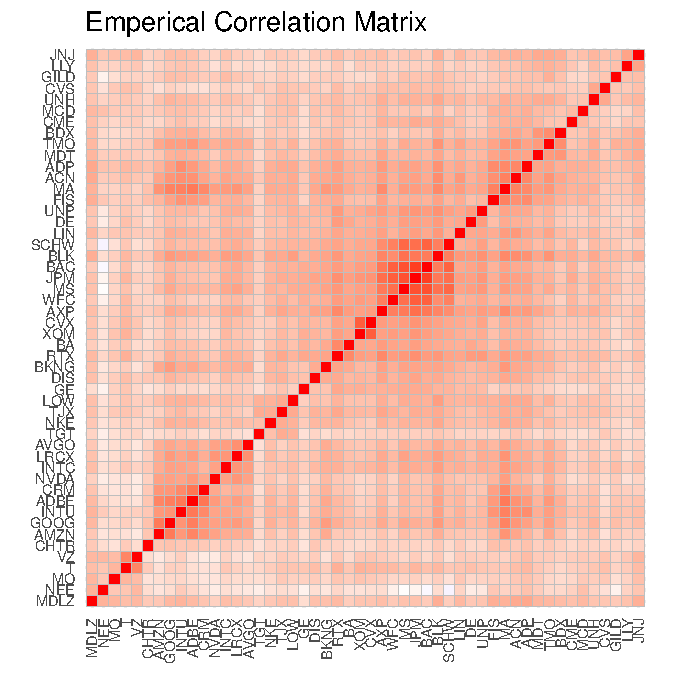
\includegraphics{Thesis_files/figure-latex/unnamed-chunk-1-1.pdf}
\caption{\label{corr_emp} Emperical Correlation Matrix}
\end{figure}

\begin{table}[!htbp] \centering 
  \caption{Eigenvalues} 
  \label{eigens} 
\begin{tabular}{@{\extracolsep{5pt}} ccccc} 
\\[-1.8ex]\hline 
\hline \\[-1.8ex] 
Diagonal & No Clusters & Five Clusters & Overlapping Clusters & Emperical \\ 
\hline \\[-1.8ex] 
1 & 15.93 & 6.4 & 14.36 & 18.6 \\ 
1 & 10.38 & 6.4 & 6.89 & 3.09 \\ 
1 & 6.28 & 6.4 & 3.3 & 2.52 \\ 
1 & 3.92 & 6.4 & 3.3 & 1.4 \\ 
1 & 2.59 & 6.4 & 2.49 & 1.28 \\ 
1 & 1.81 & 0.4 & 2.46 & 1.21 \\ 
1 & 1.32 & 0.4 & 1.3 & 1.03 \\ 
1 & 1.01 & 0.4 & 1.3 & 0.92 \\ 
1 & 0.79 & 0.4 & 1.3 & 0.88 \\ 
1 & 0.64 & 0.4 & 1.3 & 0.83 \\ 
\hline \\[-1.8ex] 
\end{tabular} 
\end{table}

\hypertarget{monte-carlo}{%
\subsection{\texorpdfstring{Monte Carlo
\label{mc}}{Monte Carlo }}\label{monte-carlo}}

A generalized version of the Monte Carlo procedure developed in Wang
\emph{et al.} (\protect\hyperlink{ref-wang2012}{2012}) was used to
simulate five distinctive market types, one type for each of the
correlation matrices discussed in Section \ref{corr_struc}. This
framework was build into the R package \emph{MCmarket} which was used to
carry out this project's Monte Carlo simulations (Potgieter,
\protect\hyperlink{ref-MCmarket}{2020}). The following briefly describes
the process:

An Elliptical t copula with 4.5 degrees of freedom was used, in
conjunction with a 50 by 50 correlation matrix, to simulate 500 random
uniformly distributed draws (corresponding to 500 trading days or
approximately two years worth of trading days) across the 50 assets. The
uniformly distributed observations were then transformed, via the
inverted normal cumulative distribution function, into normally
distributed observations (Potgieter,
\protect\hyperlink{ref-MCmarket}{2020}; Wang \emph{et al.},
\protect\hyperlink{ref-wang2012}{2012}: 3). This process was repeated 10
000 times for each of the five correlation matrices/ market types set
out in Section \ref{corr_struc}. The correlation matrix is the only
distinguishing factor between market types as all other factors remain
equal. Overall, this process created 5 data sets each containing 10 000
markets with 50 assets and 500 periods.

The expected returns and standard deviation of these simulated variables
were calibrated using a random subset of 50 of the largest 100 S\&P500
stocks between 1 January 2020 and 1 January 2021. Maximum likelihood
estimation was used to fit the multivariate t distribution to the return
series using the method developed by Liu \& Rubin
(\protect\hyperlink{ref-liu1995}{1995}). This produced a series of
estimated means and variances which were used to calibrate the expected
returns and standard deviations of the simulated variables (see Table
\ref{msd}).

\hypertarget{back-tests}{%
\subsection{\texorpdfstring{Back Tests
\label{backtest}}{Back Tests }}\label{back-tests}}

To remain consistent with the literature, as well as, the mandate for
the majority of portfolio managers, a long-only weight constraint was
applied to all portfolios. In addition, a constraint limiting the
maximum weight of a single security to 10\% is also applied. This
prevents some portfolios from building unreasonably highly concentrated
holdings, while remaining flexible enough to punish those that do so.
These constraints therefore act to provide a fair playing ground for the
portfolio's to compete. The back testing procedure works as follows.

The first 250 periods, or approximately one years worth of daily return
data, are used to fit a multivariate t distribution via maximum
likelihood and estimate a covariance matrix (Liu \& Rubin,
\protect\hyperlink{ref-liu1995}{1995}). Interestingly, the identifying
assumption used in this covariance matrix estimation method, i.e.~that
the data comes from a multivariate t distribution, is correct by
definition since this is the distribution used to simulate the data set.
The estimated covariance matrix is then used as the sole input when
calculating the weights for each of the respective risk-based
portfolios. Each portfolio holds these weights over the next 50 periods,
when they are rebalanced by looking back 250 periods, calculating a
covariance matrix and new weights. This process is repeated until all
periods in the data set are exhausted. Since there are 500 periods in
each market, each portfolio is weighted 5 times and 250 periods of daily
returns are calculated for each portfolio.

\hypertarget{portfolio-analytics}{%
\subsection{\texorpdfstring{Portfolio Analytics
\label{portmet}}{Portfolio Analytics }}\label{portfolio-analytics}}

This section describes the portfolio performance and concentration
metrics used to evaluate and compare portfolios. The Sharp ratio is used
to evaluate the risk adjusted return, while the standard deviation (SD),
downside deviation (DD) and value at risk (VaR) are used to access
portfolio risk. Finally, the effective number of constituents,
calculated as the inverse of the Herfindahl-Hirschman index (HHI), and
the effective number of bets, calculated following Meucci
(\protect\hyperlink{ref-meucci2010}{2010}), are used to compare
diversification between portfolios (Rhoades,
\protect\hyperlink{ref-rhoades1993}{1993}).

Since Markowitz (\protect\hyperlink{ref-markowitz}{1952}), the variance
of asset returns has been the standard measure for risk in the financial
industry (Meucci, \protect\hyperlink{ref-meucci2010}{2010}). SD is
simply the square-root of variance, and too is widely used as a measure
of risk. SD benefits due to its relative ease in interpretation. It is
also key in calculating the next two portfolio performance metrics
described in this study, namely the Sharp ratio and value at risk (VaR).

The Sharp ratio is a measure of a portfolio's risk adjusted returns.
Generally speaking, the Sharp ratio is calculated by dividing the
portfolio return by some measure of portfolio risk, it is therefore,
interpreted as the return per unit of risk. In this Sharp ratio is
calculated by dividing portfolio return by its standard deviation.

The 95\% VaR is another risk metric used to evaluate portfolio risk
performance in this study. It is one of the financial industry standard
measurements for downside risk and can be interpreted as the maximum
return expected from in the worst 5\% of scenarios (Peterson \& Carl,
\protect\hyperlink{ref-PerformanceAnalytics}{2020}). That is, in the
worst 5\% of scenarios, one should expect to loose at least this amount.
The particular version of VaR used here is the Gaussian VaR, this is
calculated by assuming that returns are normally distributed
\(N(\mu,\sigma)\), where \(\mu\) and \(\sigma\) are estimated using
historical data. The probability distribution assumptions enable one to
attach probability values to possible future portfolio returns. This
assumption can be dangerous in practice, however, in this study it
correct by definition, as the return series were each simulated to be
normally distributed. It should, therefore, result in an accurate
estimate of downside risk. In this study, a higher VaR is viewed as a
good thing as this implies that a smaller amount is at risk (i.e.~a VaR
of -0.01 is preferred to -0.02, where -0.01 is interpreted as being the
higher measure for VaR).

The HHI estimates portfolio concentration, and is calculated as the sum
of squared portfolio weights (Rhoades,
\protect\hyperlink{ref-rhoades1993}{1993}). A portfolio with capital
allocated evenly across a large number of securities will have an HHI of
approximately zero, while a portfolio with all its capital invested in a
single security will have the maximum HHI of 10000. The effective number
of constitutes (ENC) can then be approximated as the inverse of the HHI,
where an equally weighted portfolio with have an inverse HHI equal to
the number of securities, and more concentrated portfolios will have an
inverse HHI of less than the number of securities. Weight based measures
like the HHI are limited, in that, they are oblivious to covariation
between portfolio components. The inverse HHI can therefore, be
misleading in financial applications where portfolio components are
known to exhibit significant dependence.

Meucci (\protect\hyperlink{ref-meucci2010}{2010}) attempted to rectify
this issue when he introduced a new method to evaluate portfolio
diversification that considers portfolio risk structure. He used a
principle component (PC) approach to estimate the total number of
orthogonal bets within a portfolio, which he referred to as the
principle portfolios. With this, he estimated a portfolio
diversification distribution using the percentage of total portfolio
variation attributed to each principle portfolio. Portfolio entropy can
then be approximated as the dispersion of the diversification
distribution (Meucci, \protect\hyperlink{ref-meucci2010}{2010}: 10). In
this context entropy can be interpreted as the effective number of
orthogonal bets within a portfolio.

\hypertarget{results-and-discussion}{%
\section{\texorpdfstring{Results and Discussion
\label{reasults}}{Results and Discussion }}\label{results-and-discussion}}

This section has two main parts, the first (Section
\ref{within-market}), compares the relative performance of the five
risk-based portfolios in each of the five market types, and the second
(Section \ref{cross-market}), investigates how each portfolio's relative
performance changes across the market types. But first, a short note
discussing some interesting trends and caveats regarding the portfolio
concentration measures.

\hypertarget{a-note-on-the-potfolio-concerntration-metrics}{%
\paragraph{A Note on the Potfolio Concerntration
Metrics}\label{a-note-on-the-potfolio-concerntration-metrics}}

The average inverse HHI and entropy for each portfolio, across the five
market types can be found in Tables \ref{rm1}, \ref{rm2}, \ref{rm3},
\ref{rm4} and \ref{rm5}. Throughout the five market types, the inverse
HHI and entropy measures are typically at odds. Portfolio's rated as
highly diversified by the inverse HHI are are rated as relatively
undiversified in entropy and \emph{vice verse}. An interesting
observation is that the inverse HHI measure better coincides with the
other portfolio risk measures.

Furthermore, when ranked in order of concentration score, the results
tend to be consistent across the five market types. The EW's inverse HHI
is the highest in all five market types and its entropy is the lowest.
Conversely, the MV portfolio's inv HHI is the lowest in all Market
types, while its entropy tends to be one of the highest. The IV
portfolio typically ranks second for the highest inverse HHI, and lowest
entropy. The ERC has the third highest inverse HHI and third highest
entropy. The MD has the second lowest HHI, while its entropy
consistently ranks as on of the highest. Overall, this indicates that
the EW, IV and ERC portfolios diversify well across assets and poorly
across risk sources, while the MD and MV portfolios diversify poorly
across assets and well across sources of risk.

\hypertarget{comparing-portfolios-within-market-types}{%
\subsection{\texorpdfstring{Comparing Portfolios Within Market Types
\label{within-market}}{Comparing Portfolios Within Market Types }}\label{comparing-portfolios-within-market-types}}

\hypertarget{market-1}{%
\subsubsection{Market 1}\label{market-1}}

The portfolios compared here were evaluated within the markets simulated
using the 'Diagonal Matrix" (Figure \ref{corr_mats}). Due to the lack of
dependence between its constituents, this market type is arguable the
least realistic. According to the portfolio average Sharp ratio, SD, DD
and VaR measures the EW portfolio performed the best overall (Table
\ref{rm1}). The IV portfolio was a close second, it has the second
highest Sharp ratio, tied the lowest SD, and is ranked second in the DD
and VaR metrics. The ERC ranked the third best overall, followed by the
MD and finally the MV.

\begin{table}[!htbp] \centering 
  \caption{Market 1 - Portfolio Risk Metrics} 
  \label{rm1} 
\begin{tabular}{@{\extracolsep{5pt}} cccccc} 
\\[-1.8ex]\hline 
\hline \\[-1.8ex] 
Metric & EW & MV & IV & ERC & MD \\ 
\hline \\[-1.8ex] 
Sharp & 0.19353 & 0.13501 & 0.18341 & 0.15876 & 0.14284 \\ 
SD & 0.00386 & 0.005 & 0.00386 & 0.00447 & 0.00494 \\ 
Downside Deviation & 0.00235 & 0.00318 & 0.00236 & 0.00279 & 0.00312 \\ 
VaR & -0.00545 & -0.00735 & -0.00548 & -0.00645 & -0.00722 \\ 
Inv HHI & 50 & 27.2 & 47.3 & 35.6 & 28.2 \\ 
Entropy & 17.5 & 22.8 & 20.1 & 18.9 & 21 \\ 
\hline \\[-1.8ex] 
\end{tabular} 
\end{table}

The EW portfolio ranked first overall in Sharp ratio, SD, DD and VaR.
The IV portfolio lagged just behind, ranking second overall across the
measures. The ERC was ranked third across the aforementioned metrics,
followed by the MD and finally the MV.

Since Market 1 has real no correlation structure it is unsurprising that
the two portfolios that neglect using covariance information have
performed relatively well. The EW and IV portfolios effectively assume
that there is no correlation between assets. In Market 1 this assumption
is correct by construction. However, since the variance does differ
between assets it would have been reasonable to assume that the IV
portfolio would be the least volatile. The fact that it is not may be
because asset return variances are not sufficiently different to punish
the EW ignorance and/or the IV portfolio's out of sample variance
forecast is not accurate enough to effectively reduce risk out of
sample.

The MV, ERC and MD portfolios performed poorly compared to the EW and IV
portfolios. This is likely be due to there being no real dependence in
the underlying market's correlation structure. Therefore, these
portfolios are more noisy in comparison, and likely use spurious
covariance information when allocating capital. Out of the three the ERC
portfolio is the best by a wide margin.

\hypertarget{market-2}{%
\subsubsection{Market 2}\label{market-2}}

The portfolios compared here were evaluated within the markets simulated
using the `No Clusters' correlation matrix (Figure \ref{corr_mats}).
Unlike in Market 1 the portfolio risk metrics in Table \ref{rm2} do not
rank the portfolios in a clear order. Despite having the highest average
SD, the MD portfolio achieved the highest Sharp ratio. The ERC performed
best in the SD, DD and VaR measures while obtaining the second highest
Sharp ratio. The EW and IV portfolios were similar in their performance
and the MV performed poorly.

\begin{table}[!htbp] \centering 
  \caption{Market 2 - Portfolio Risk Metrics} 
  \label{rm2} 
\begin{tabular}{@{\extracolsep{5pt}} cccccc} 
\\[-1.8ex]\hline 
\hline \\[-1.8ex] 
Metric & EW & MV & IV & ERC & MD \\ 
\hline \\[-1.8ex] 
Sharp & 0.05158 & 0.03432 & 0.04948 & 0.053 & 0.06484 \\ 
SD & 0.01454 & 0.01446 & 0.01438 & 0.01431 & 0.01508 \\ 
Downside Deviation & 0.00985 & 0.00993 & 0.00976 & 0.00969 & 0.01011 \\ 
VaR & -0.02276 & -0.02289 & -0.02255 & -0.02238 & -0.02338 \\ 
Inv HHI & 50 & 12.2 & 47.5 & 47.4 & 13.9 \\ 
Entropy & 1.1 & 1.8 & 1.1 & 1.2 & 2 \\ 
\hline \\[-1.8ex] 
\end{tabular} 
\end{table}

In Market 2, the MV portfolio has the lowest overall Sharp ratio, the
third highest SD, the second highest DD and the worst VaR. Despite it
managing to attain a fairly low average SD, its poor performance across
the other risk measures (i.e.~DD and VaR) demonstrates a crucial failure
to mitigate downside risk exposure. Critically, the mitigation of
downside risk is arguably more important than simply reducing
volatility. Its low sharp ratio indicates that it was not well
compensated for holding its risk and performed exceedingly poorly from a
total return perspective. Its entropy score indicates that it is
diversified relatively well across risk sources. However, its inverse
HHI suggests that it is highly concentrated in a few number of assets
(Table \ref{rm2}).

The EW and IV portfolios performed very similarly in Market 2. This is a
recurring theme thought the market types (for example see Tables
\ref{rm3} and \ref{rm4}). The EW has the higher Sharp ratio of the two,
while the IV performs better in the SD, DD and VaR measures. Therefore,
it seems like the the EW portfolio finds itself sightly closer to the
top right quadrant of the efficient frontier, where it earns higher
returns with greater risk compared to the IV portfolio. Both portfolios
have a high inverse HHI, indicating that they were well diversified
across assets. While, in comparison to the other portfolios, they have a
low entropy measure and are therefore, are not well diversified across
risk sources. This has however, not translated into higher average
portfolio volatility.

The MD portfolio acts as Market 2's wild card. It has the highest
average Sharp ratio by a significant margin, but performs the worst in
the SD and DD risk metrics. Despite it having the largest SD, the MD is
on par with the best VaR. This indicates that, compared to the other
portfolios, the MD earned exceptionally high returns. Interestingly, it
has the highest entropy score and is therefore well diversified across
risk sources. Comparatively, it has a low inverse HHI and is therefore,
highly concentrated in a small number of assets.

Compared to the MD portfolio, the ERC seems to be safer and consistent.
The ERC scored the best overall across the three risk metrics and
achieved the second highest Sharp ratio. Therefore, from a risk
mitigation perspective the ERC is the clear winner. However, the high
returns obtained by the MD portfolio may entice less risk averse
investors. Compared to the MD, the ERC is well diversified across assets
and poorly diversified across risk sources.

\hypertarget{market-3}{%
\subsubsection{Market 3}\label{market-3}}

The portfolios compared here were evaluated within the markets simulated
using the `Five Clusters' correlation matrix (Figure \ref{corr_mats}).
This market structure has not produced a clear winner. On average the
EW, IV, ERC and MD portfolios performed quite similarly, meanwhile, the
MV portfolio is the clear looser. The MV is the worst performer across
the Sharp, SD, DD and VaR measures (Table \ref{rm3}). The IV and ERC
portfolios performed very similarly. The EW portfolio the highest
average Sharp ratio and maintains relatively low risk. The MD portfolio
performed poorly compared to the EW, IV and ERC portfolios, but still
outperformed the MV by a comfortable margin.

\begin{table}[!htbp] \centering 
  \caption{Market 3 - Portfolio Risk Metrics} 
  \label{rm3} 
\begin{tabular}{@{\extracolsep{5pt}} cccccc} 
\\[-1.8ex]\hline 
\hline \\[-1.8ex] 
Metric & EW & MV & IV & ERC & MD \\ 
\hline \\[-1.8ex] 
Sharp & 0.07949 & 0.05165 & 0.07608 & 0.07602 & 0.07098 \\ 
SD & 0.00941 & 0.01034 & 0.00932 & 0.00933 & 0.01011 \\ 
Downside Deviation & 0.00625 & 0.00701 & 0.0062 & 0.00621 & 0.00675 \\ 
VaR & -0.01439 & -0.01613 & -0.01428 & -0.0143 & -0.01555 \\ 
Inv HHI & 50 & 14.6 & 47.6 & 46 & 17.8 \\ 
Entropy & 1.3 & 3.7 & 1.4 & 1.5 & 2.2 \\ 
\hline \\[-1.8ex] 
\end{tabular} 
\end{table}

In Market 3, the EW portfolio has the third lowest SD, DD and VaR.
Therefore, despite there being significant and distinct risk clusters in
the underlying market structure the EW portfolio achieved a relatively
high level of diversification. It has the highest average Sharp ratio,
suggesting that it performed well from a total return stand point.
According to its entropy measure, it is the least diversified across
risk sources. The above findings hold in Markets 3, 4 and 5 and will
therefore not be repeated (see Tables \ref{rm4} and \ref{rm5}).

On average the MV portfolio performed exceedingly poorly, its has the
lowest Sharp ratio by far and is the worst performer across the SD, DD
and VaR measures. Its inability to maintain a low average out of sample
SD indicates that it suffers from estimation error. The inverse HHI and
entropy metrics in Table \ref{rm3} indicate that the MV portfolio is the
least diversified across assets and the most diversified across sources
of risk. These findings hold in Market 4 and are not repeated (see
\ref{rm4}).

The IV and ERC portfolios were strong contenders for first place. Their
scores were close across all 6 measures (Table \ref{rm3}). They were
about equal in their ability to mitigate risk. The IV has a slightly
lower SD, the ERC slightly lower DD and the IV slightly higher VaR.
Their Sharp ratios also seem to suggest that they were fairly well
compensated for holding risk. Their respective inverse HHI and entropy
scores indicate that they are well diversified across assets and poorly
diversified across risk sources.

The MD portfolio performed worse than the EW, IV and ERC portfolios. It
has a lower Sharp ratio, higher SD, DD and a lower VaR. However, it
underperformed these portfolios by a fairly small margin, and did
substantially better than the MV portfolio in this regard. It is
relatively highly concentrated across assets and fairly well diversified
across risk sources.

\hypertarget{market-4}{%
\subsubsection{Market 4}\label{market-4}}

The portfolios compared here were evaluated within the markets simulated
using the `Overlapping Clusters' correlation matrix (Figure
\ref{corr_mats}). There is therefore, a positive correlation coefficient
between all assets in the underlying correlation structure. Despite this
the EW and IV portfolios, which are oblivious to asset covariance,
managed significant risk reduction. The IV and ERC portfolios performed
about equally well across all the metrics in Table \ref{rm4}. The MV
performed the worst, the MD narrowly outperformed it in the SD, DD and
VaR measures.

\begin{table}[!htbp] \centering 
  \caption{Market 4 - Portfolio Risk Metrics} 
  \label{rm4} 
\begin{tabular}{@{\extracolsep{5pt}} cccccc} 
\\[-1.8ex]\hline 
\hline \\[-1.8ex] 
Metric & EW & MV & IV & ERC & MD \\ 
\hline \\[-1.8ex] 
Sharp & 0.05368 & 0.03225 & 0.05155 & 0.05154 & 0.05006 \\ 
SD & 0.01397 & 0.01447 & 0.0138 & 0.0138 & 0.01443 \\ 
Downside Deviation & 0.00946 & 0.00996 & 0.00935 & 0.00936 & 0.00979 \\ 
VaR & -0.02184 & -0.02294 & -0.02159 & -0.0216 & -0.0226 \\ 
Inv HHI & 50 & 13 & 47.6 & 46.7 & 13.7 \\ 
Entropy & 1.1 & 2 & 1.1 & 1.1 & 1.6 \\ 
\hline \\[-1.8ex] 
\end{tabular} 
\end{table}

The IV and ERC performed very similarly in this market. They are
approximately tied as the best performing portfolios across the SD, DD
and VaR measures. They are also approximately tie with the second
highest Sharp ratio. They are both well diversified across assets, but
relatively highly concentrated across risk sources (Table \ref{rm4}).

The MD portfolio is the second worst performing portfolio in Market 2.
It ranks second to last across Sharp ratio, SD, DD and VaR metrics
(Table \ref{rm4}). Its Sharp ratio is not substantially lower than that
of the IV and ERC, thereby indicating that the MD was compensated fairly
for holding risk. The MD has a relatively low inverse HHI and has the
the highest entropy.

\hypertarget{market-5}{%
\subsubsection{Market 5}\label{market-5}}

The portfolios compared here were evaluated within the markets simulated
using the `Empirical Correlation Matrix' (Figure \ref{corr_emp}). This
is therefore, the most realistic of the five correlation matrices. It
exhibits significant correlation between assets, with some noticeable
risk clusters. The IV and ERC portfolios performed similarly across all
metrics (Table \ref{rm5}). The MV and MD portfolios performed the worst.
The EW has the highest sharp ratio, but was out performed by the IV and
ERC in terms of risk mitigation.

\begin{table}[!htbp] \centering 
  \caption{Market 5 - Portfolio Risk Metrics} 
  \label{rm5} 
\begin{tabular}{@{\extracolsep{5pt}} cccccc} 
\\[-1.8ex]\hline 
\hline \\[-1.8ex] 
Metric & EW & MV & IV & ERC & MD \\ 
\hline \\[-1.8ex] 
Sharp & 0.04708 & 0.03473 & 0.04526 & 0.04511 & 0.04556 \\ 
SD & 0.01585 & 0.01684 & 0.01564 & 0.01579 & 0.0171 \\ 
Downside Deviation & 0.01078 & 0.01157 & 0.01065 & 0.01076 & 0.01164 \\ 
VaR & -0.02497 & -0.02676 & -0.02466 & -0.0249 & -0.02697 \\ 
Inv HHI & 50 & 13 & 47.5 & 43.6 & 12.5 \\ 
Entropy & 1.1 & 1.6 & 1.2 & 1.2 & 1.5 \\ 
\hline \\[-1.8ex] 
\end{tabular} 
\end{table}

In Market 5 the MV portfolio has the lowest Sharp ratio and ranked
second worst in the SD, DD and VaR measures. It therefore, failed in its
objective to minimize portfolio volatility, and the relatively simple EW
and IV portfolios outperformed it in this regard. Its out of sample
performance is therefore, suffering due to estimation error. Its inverse
HHI indicates that it is highly concentrated in a relatively small
number of assets. Conversely, its entropy suggests it is the most
successful portfolio in diversifying across risk sources.

The IV portfolio has the third highest Sharp ratio, the lowest SD, the
second lowest DD and the highest VaR and narrowly outperformed the ERC
in all the aforementioned metrics. Furthermore, the IV portfolio is well
diversified across assets, as shown by its inverse HHI, meanwhile, its
entropy score suggests it is comparatively less diversified across risk
sources.

The MD portfolio received the second highest Sharp ratio, the highest SD
and DD, and performed the worst in VaR. Its inverse HHI indicates that
it is highly concentrated in a small number of assets, while its entropy
suggests that it has done relatively well in diversifying across risk
sources.

\hypertarget{comparing-portfolios-across-market-types}{%
\subsection{\texorpdfstring{Comparing Portfolios Across Market Types
\label {cross-market}}{Comparing Portfolios Across Market Types }}\label{comparing-portfolios-across-market-types}}

This section compares the relative portfolio performance across the five
market types, thereby, investigating the link between correlation
structure and portfolio performance. Each portfolio's standardized Sharp
ratio, SD, DD, and VaR performance metrics, as well as, their inverse
HHI and entropy scores, across the five market types are provided in
tables \ref{ew}, \ref{mv}, \ref{iv}, \ref{erc} and \ref{md}. Values were
standardized via the usual z-score transformation and can therefore, be
interpreted as standard deviations. Section \ref{entropych} discusses
how each portfolios entropy changes between the five markets and Section
\ref{perf} discusses the relative portfolio performance across market
types,

\hypertarget{entropy-across-market-types}{%
\subsubsection{\texorpdfstring{Entropy Across Market Types
\label{entropych}}{Entropy Across Market Types }}\label{entropy-across-market-types}}

All portfolios had their highest entropy score in Market 1 an second
highest in Market three. These markets simply had the most scope for
diversification. Therefore, the interesting changes in entropy occur
between markets 2, 4 and 5. When moving from Market 2 to 4, the EW, IV,
ERC and MD portfolios experienced a decline in their entropy score,
while the MV portfolio's entropy improved. Looking at the change in
entropy when moving from Market 2 to Market 5, the IV and ERC experience
improvements and the EW, MV, and MD declines. Finally, when moving from
Market 4 to 5, the EW, IV, ERC and MD all experience improvements, while
the the MV suffers a decline.

\hypertarget{performance-metrics-across-market-types}{%
\subsubsection{\texorpdfstring{Performance Metrics Across Market Types
\label{perf}}{Performance Metrics Across Market Types }}\label{performance-metrics-across-market-types}}

\begin{table}[!htbp] \centering 
  \caption{Equal Weight} 
  \label{ew} 
\begin{tabular}{@{\extracolsep{5pt}} cccccc} 
\\[-1.8ex]\hline 
\hline \\[-1.8ex] 
Metric & Market 1 & Market 2 & Market 3 & Market 4 & Market 5 \\ 
\hline \\[-1.8ex] 
Sharp & 1.2192 & 0.0858 & 0.7753 & 0.6666 & 0.7076 \\ 
SD & -1.0181 & -0.0457 & -0.6014 & -0.3728 & -0.5851 \\ 
Downside Deviation & -1.029 & -0.1105 & -0.6266 & -0.4497 & -0.6218 \\ 
VaR & 1.0309 & 0.0837 & 0.6304 & 0.4427 & 0.6113 \\ 
Inv HHI & 50 & 50 & 50 & 50 & 50 \\ 
Entropy & 20.362 & 1.3586 & 3.2539 & 1.101 & 1.1167 \\ 
\hline \\[-1.8ex] 
\end{tabular} 
\end{table}

The EW portfolio performed better than average, across all five market
types, in the Sharp ratio, SD, DD and VaR metrics. According to the
standardized scores in Table \ref{ew}, the EW portfolio performed best
in Market 1, followed by Market 3, Market 5 and finally, Market 2. As
previously mentioned, its excellent Market 1 performance is
unsurprising. However, its ability to achieve substantial risk reduction
in markets characterized by significant dependence, demonstrates the
effectiveness of this simple strategy. Its relative performance across
markets indicates that it exceeds in markets with little or no
correlation between assets and maintains its success through a variety
of market structures.

The EW's inverse HHI is by construction equal to 50 in all markets,
while its entropy declined with the number of correlated assets. The
decline in entropy is simply due to a decrease in the scope for
diversification and is therefore, experienced across all portfolios.

\begin{table}[!htbp] \centering 
  \caption{Minimum Variance} 
  \label{mv} 
\begin{tabular}{@{\extracolsep{5pt}} cccccc} 
\\[-1.8ex]\hline 
\hline \\[-1.8ex] 
Metric & Market 1 & Market 2 & Market 3 & Market 4 & Market 5 \\ 
\hline \\[-1.8ex] 
Sharp & -1.0958 & -1.4968 & -1.7213 & -1.7695 & -1.7667 \\ 
SD & 1.0325 & -0.3068 & 1.3139 & 1.1305 & 0.885 \\ 
Downside Deviation & 1.0541 & 0.3807 & 1.4084 & 1.3636 & 1.0157 \\ 
VaR & -1.0528 & -0.2563 & -1.4008 & -1.3346 & -0.9931 \\ 
Inv HHI & 27.4705 & 11.4806 & 14.0377 & 12.2394 & 12.1014 \\ 
Entropy & 21.9552 & 2.0646 & 5.3911 & 2.2467 & 1.7717 \\ 
\hline \\[-1.8ex] 
\end{tabular} 
\end{table}

The MV portfolio performs below average across all five markets. It
scores approximately one standard deviation below average in the Sharp
ratio, SD, DD and VaR metrics in Markets 1, 3 and 4. Its Sharp ratio is
at least one standard deviation below average in all five markets. It
performed best in Market 2, however, even then it performed below
average in Sharp ratio, DD and VaR. Therefore, across all of the market
types the MV portfolio's out of sample performance suffered due to
estimation error.

\begin{table}[!htbp] \centering 
  \caption{Inverse Volatility} 
  \label{iv} 
\begin{tabular}{@{\extracolsep{5pt}} cccccc} 
\\[-1.8ex]\hline 
\hline \\[-1.8ex] 
Metric & Market 1 & Market 2 & Market 3 & Market 4 & Market 5 \\ 
\hline \\[-1.8ex] 
Sharp & 0.8189 & -0.1067 & 0.4696 & 0.4245 & 0.343 \\ 
SD & -1.0181 & -0.5679 & -0.7867 & -0.8839 & -0.8969 \\ 
Downside Deviation & -1.0039 & -0.6632 & -0.7604 & -0.8486 & -0.8913 \\ 
VaR & 0.998 & 0.633 & 0.7588 & 0.8466 & 0.8891 \\ 
Inv HHI & 47.2773 & 47.3 & 47.2838 & 47.287 & 47.2623 \\ 
Entropy & 21.2181 & 1.3726 & 3.3521 & 1.1399 & 1.1482 \\ 
\hline \\[-1.8ex] 
\end{tabular} 
\end{table}

Across the five markets, the IV portfolio performed above average in SD,
DD and VaR. The IV portfolio performed best in Market 1, and worst in
Market 2. Its Sharp ratio in Market 2 is the only occasion it performed
above average average. Overall the IV portfolio proved to be successful
and robust across market types. Based on its relative performance across
markets it seems to strive in markets with little or no correlation
between assets, but maintains its success through a variety of market
structures.

\begin{table}[!htbp] \centering 
  \caption{Equal Risk Contribution} 
  \label{erc} 
\begin{tabular}{@{\extracolsep{5pt}} cccccc} 
\\[-1.8ex]\hline 
\hline \\[-1.8ex] 
Metric & Market 1 & Market 2 & Market 3 & Market 4 & Market 5 \\ 
\hline \\[-1.8ex] 
Sharp & -0.1563 & 0.216 & 0.4642 & 0.4233 & 0.3129 \\ 
SD & 0.0791 & -0.7963 & -0.7661 & -0.8839 & -0.6741 \\ 
Downside Deviation & 0.0753 & -1.093 & -0.7337 & -0.8124 & -0.6633 \\ 
VaR & -0.0658 & 1.0776 & 0.7354 & 0.8305 & 0.674 \\ 
Inv HHI & 35.9119 & 46.3298 & 44.9382 & 46.1096 & 42.7687 \\ 
Entropy & 21.1598 & 1.4843 & 3.3722 & 1.1407 & 1.1584 \\ 
\hline \\[-1.8ex] 
\end{tabular} 
\end{table}

In Markets 2, 3, 4 and 5 the ERC portfolio performed above average in
Sharp Ratio, SD, DD and VaR. In Market 1 its performance was mediocre,
scoring below average in Sharp ratio and VaR and above average in SD and
DD. It performed best, from a downside risk mitigation perspective in
Market 2 (see DD and VaR). Overall, it seems like Market 1 not a good
match for the ERC, however, across Markets 2, 3, 4 and 5 its relative
performance was fairly consistent. This suggests that the ERC is able to
perform well across a variety of markets with significant correlation
between their assets. This describes practically all real world asset
markets.

\begin{table}[!htbp] \centering 
  \caption{Maximum Diversification} 
  \label{md} 
\begin{tabular}{@{\extracolsep{5pt}} cccccc} 
\\[-1.8ex]\hline 
\hline \\[-1.8ex] 
Metric & Market 1 & Market 2 & Market 3 & Market 4 & Market 5 \\ 
\hline \\[-1.8ex] 
Sharp & -0.786 & 1.3016 & 0.0122 & 0.2551 & 0.4031 \\ 
SD & 0.9245 & 1.7167 & 0.8403 & 1.0102 & 1.2711 \\ 
Downside Deviation & 0.9035 & 1.486 & 0.7122 & 0.7471 & 1.1608 \\ 
VaR & -0.9102 & -1.538 & -0.7237 & -0.7852 & -1.1813 \\ 
Inv HHI & 29.1668 & 12.8975 & 16.211 & 14.2876 & 13.2099 \\ 
Entropy & 21.1969 & 2.3394 & 4.5327 & 1.5828 & 1.6707 \\ 
\hline \\[-1.8ex] 
\end{tabular} 
\end{table}

From a risk mitigation perspective, the MD portfolio consistently
performed well below average. It has a standardized score of greater
than 0.7 for SD and DD, and less that -0.7 for VaR. Meanwhile, it
managed to achieve above average Sharp ratios in Markets 2, 3 , 4 and 5,
suggesting that made returns well above average in these markets. In
Markets 1, 3 and 4, the MD portfolio performed quite poorly across all
measures. In Market 2 it received the highest standardized Sharp ratio
while performing its worst across the SD, DD and VaR measures. In Market
5 it has a fairly good Sharp ratio, but had poor risk mitigation (see
SD, DD and VaR). Overall, it doesn't see, like any of the market
structures were a particularly good match for the MD portfolio.

\hypertarget{discussion}{%
\subsection{Discussion}\label{discussion}}

The MV portfolio continued to perform well below average in all market
types (Table \ref{mv}). It struggled to maintain out of sample low
volatility and seemed to be particularly bad at mitigating downside
risk. It consistently received the lowest Sharp ratio, indicating that
on average it returned less than the other portfolios. It low average
inverse HHI and high average entropy indicate that it diversifies well
across sources fo risk by concentrating its holdings in a small number
of assets.

The EW and IV portfolios performed above average in all measures, across
all market types. They both performed their best in Market 1, worst in
Market 2. In Markets 3, 4 an 5 the IV portfolio outperformed the MV form
a risk mitigation perspective, however, the EW achieved a highers Sharp
ratio (Tables \ref{ew} and \ref{iv}). They both exhibit high
diversification across assets, but fail to diversify across sources of
risk.

The ERC portfolio showed above average performance in Markets 2, 3, 4
and 5. It performed its worst in Market 1 and seemed to improve in
markets with higher condition numbers. It was about equal to the IV
portfolio in Markets 3, 4 and 5, but outperformed the IV in Market 2. Is
concentration scores indicate that it diversifies across assets better
than what it does across risk sources. It does, however, show
improvement over the EW and IV in its diversification across risk
sources.

The MD portfolio's performance was often mixed within markets, however,
it was clearly at its worst in Market 1. In Markets 2 and 5, it showed
great promise in its ability to earn a high Sharp ratio, but at the same
time struggled to keep its SD and DD down. This characteristic proved to
quite interesting, in that, it often scored exceptionally well in its
Sharp ratio, whilst performing exceedingly poorly in risk mitigation
(for example see Market 2). It would be interesting to investigate if
this high risk high reward attribute holds in other Monte Carlo
environments. The MD portfolio's concentration scores suggest that it
diversifies well across risk sources and poorly across assets.

\hypertarget{conclusion}{%
\section{\texorpdfstring{Conclusion
\label{conclusion}}{Conclusion }}\label{conclusion}}

This work used Monte Carlo methods to calculate the returns of five
risk-based portfolios across a set of five unique market types, thereby,
enabling a the successful and comprehensive comparison of said
portfolios relative performance across each market type. Overall, the EW
and IV portfolios performed well across a range of market types, while
the ERC performed well in those with a high condition number. In all
market types, the MV portfolio proved unable to maintain low out of
sample volatility and performed poorly from a total return perspective.
Thereby demonstrating that it is sensitive to estimation error in the
covariance matrix. The EW and IV portfolios were found to perform above
average across all market types. They performed their best in the market
with the ``Diagonal Matrix'' correlation structure and their worst in
the worst in the market with the ``No Clusters'' correlation matrix. The
ERC portfolio performed poorly in the market with the ``Diagonal
Matrix'' correlation structure and its performance improved in markets
with higher condition number correlation matrices. In markets with
significant correlations in their market structure the ERC and IV
performed similarly. In all market types, the MD portfolio proved to be
unsuccessful in reducing volatility, however, in some market structures
it showed potential to achieve a high average Sharp ratio. The average
inverse HHI and entropy measures showed that the EW, IV and ERC
portfolios diversify well across assets and poorly across risk sources.
Conversely, the MV and MD portfolios diversify well across risk sources
and poorly across assets. These results indicate the potential for
incorporating simple heuristic approaches, like those of the EW and IV
portfolios, in the development of future risk-based portfolio
algorithms.

\newpage

\hypertarget{references}{%
\section*{References}\label{references}}
\addcontentsline{toc}{section}{References}

\hypertarget{refs}{}
\leavevmode\hypertarget{ref-ardia2017}{}%
Ardia, D., Bolliger, G., Boudt, K. \& Gagnon-Fleury, J.-P. 2017. The
impact of covariance misspecification in risk-based portfolios.
\emph{Annals of Operations Research}. 254(1-2):1--16.

\leavevmode\hypertarget{ref-lopez2012}{}%
Bailey, D.H. \& Lopez De Prado, M. 2012. Balanced baskets: A new
approach to trading and hedging risks. \emph{Journal of Investment
Strategies (Risk Journals)}. 1(4).

\leavevmode\hypertarget{ref-Matrix}{}%
Bates, D. \& Maechler, M. 2019. \emph{Matrix: Sparse and dense matrix
classes and methods}. ed. {[}Online{]}, Available:
\url{https://CRAN.R-project.org/package=Matrix}.

\leavevmode\hypertarget{ref-choueifaty2008}{}%
Choueifaty, Y. \& Coignard, Y. 2008. Toward maximum diversification.
\emph{The Journal of Portfolio Management}. 35(1):40--51.

\leavevmode\hypertarget{ref-choueifaty2013}{}%
Choueifaty, Y., Froidure, T. \& Reynier, J. 2013. Properties of the most
diversified portfolio. \emph{Journal of investment strategies}.
2(2):49--70.

\leavevmode\hypertarget{ref-clarke2011}{}%
Clarke, R., De Silva, H. \& Thorley, S. 2011. Minimum-variance portfolio
composition. \emph{The Journal of Portfolio Management}. 37(2):31--45.

\leavevmode\hypertarget{ref-leote}{}%
De Carvalho, R.L., Lu, X. \& Moulin, P. 2012a. Demystifying equity
risk--based strategies: A simple alpha plus beta description. \emph{The
Journal of Portfolio Management}. 38(3):56--70.

\leavevmode\hypertarget{ref-rawl2012}{}%
De Carvalho, R.L., Lu, X. \& Moulin, P. 2012b. Demystifying equity
risk--based strategies: A simple alpha plus beta description. \emph{The
Journal of Portfolio Management}. 38(3):56--70.

\leavevmode\hypertarget{ref-demiguel2009}{}%
DeMiguel, V., Garlappi, L. \& Uppal, R. 2009. Optimal versus naive
diversification: How inefficient is the 1/n portfolio strategy?
\emph{The review of Financial studies}. 22(5):1915--1953.

\leavevmode\hypertarget{ref-lopez}{}%
De Prado, M.L. 2016. Building diversified portfolios that outperform out
of sample. \emph{The Journal of Portfolio Management}. 42(4):59--69.

\leavevmode\hypertarget{ref-fama1992}{}%
Fama, E.F. \& French, K.R. 1992. The cross-section of expected stock
returns. \emph{the Journal of Finance}. 47(2):427--465.

\leavevmode\hypertarget{ref-glasserman2013}{}%
Glasserman, P. 2013. \emph{Monte carlo methods in financial
engineering}. ed. Vol. 53. Springer Science \& Business Media.

\leavevmode\hypertarget{ref-higham2002}{}%
Higham, N.J. 2002. Computing the nearest correlation matrix---a problem
from finance. \emph{IMA journal of Numerical Analysis}. 22(3):329--343.

\leavevmode\hypertarget{ref-kroese2014}{}%
Kroese, D.P., Brereton, T., Taimre, T. \& Botev, Z.I. 2014. Why the
monte carlo method is so important today. \emph{Wiley Interdisciplinary
Reviews: Computational Statistics}. 6(6):386--392.

\leavevmode\hypertarget{ref-liu1995}{}%
Liu, C. \& Rubin, D.B. 1995. ML estimation of the t distribution using
em and its extensions, ecm and ecme. \emph{Statistica Sinica}. 19--39.

\leavevmode\hypertarget{ref-maillard2010}{}%
Maillard, T., Roncalli. 2010. The properties of equally weighted risk
contribution portfolios. \emph{The Journal of Portfolio Management}.
36(4):60--70.

\leavevmode\hypertarget{ref-markowitz}{}%
Markowitz, H. 1952. Portfolio selection. \emph{The Journal of Finance}.
7(1):77--91.

\leavevmode\hypertarget{ref-meucci2010}{}%
Meucci, A. 2010. Managing diversification.

\leavevmode\hypertarget{ref-fitHeavyTail}{}%
Palomar, D.P. \& ZHOU, R. 2020. \emph{fitHeavyTail: Mean and Covariance
Matrix Estimation under Heavy Tails}. ed. {[}Online{]}, Available:
\url{https://CRAN.R-project.org/package=fitHeavyTail}.

\leavevmode\hypertarget{ref-perold2004}{}%
Perold, A.F. 2004. The capital asset pricing model. \emph{Journal of
economic perspectives}. 18(3):3--24.

\leavevmode\hypertarget{ref-PerformanceAnalytics}{}%
Peterson, B.G. \& Carl, P. 2020. \emph{PerformanceAnalytics: Econometric
tools for performance and risk analysis}. ed. {[}Online{]}, Available:
\url{https://CRAN.R-project.org/package=PerformanceAnalytics}.

\leavevmode\hypertarget{ref-MCmarket}{}%
Potgieter, N. 2020. \emph{MCmarket: Package to simplify the monte carlo
simulation of financial markets}. ed. Stellenbosch, South Africa:
Stellenbosch University.

\leavevmode\hypertarget{ref-rhoades1993}{}%
Rhoades, S.A. 1993. The herfindahl-hirschman index. \emph{Fed. Res.
Bull.} 79:188.

\leavevmode\hypertarget{ref-tu2011}{}%
Tu, J. \& Zhou, G. 2011. Markowitz meets talmud: A combination of
sophisticated and naive diversification strategies. \emph{Journal of
Financial Economics}. 99(1):204--215.

\leavevmode\hypertarget{ref-wang2012}{}%
Wang, P., Sullivan, R.N. \& Ge, Y. 2012. Risk-based dynamic asset
allocation withExtreme tails and correlations. \emph{The Journal of
Portfolio Management}. 38(4):26--42.

\leavevmode\hypertarget{ref-zhou2019}{}%
Zhou, R., Liu, J., Kumar, S. \& Palomar, D.P. 2019. Robust factor
analysis parameter estimation. In ed. Springer \emph{International
conference on computer aided systems theory}. 3--11.

\newpage

\hypertarget{appendix}{%
\section*{Appendix}\label{appendix}}
\addcontentsline{toc}{section}{Appendix}

\begin{table}[!htbp] \centering 
  \caption{Asset Means and Sd's} 
  \label{msd} 
\begin{tabular}{@{\extracolsep{5pt}} cccccc} 
\\[-1.8ex]\hline 
\hline \\[-1.8ex] 
Asset & Mean & Sd & Asset... & Mean... & Sd... \\ 
\hline \\[-1.8ex] 
Asset\_1 & -0.00011 & 0.03277 & Asset\_26 & 0.00247 & 0.02671 \\ 
Asset\_2 & 0.00023 & 0.02314 & Asset\_27 & -0.00132 & 0.04888 \\ 
Asset\_3 & -3e-05 & 0.02359 & Asset\_28 & 0.00085 & 0.02387 \\ 
Asset\_4 & -0.0018 & 0.03654 & Asset\_29 & 0.00024 & 0.01613 \\ 
Asset\_5 & -0.00036 & 0.02925 & Asset\_30 & 0.00086 & 0.01884 \\ 
Asset\_6 & 0.00052 & 0.02396 & Asset\_31 & 0.00118 & 0.03147 \\ 
Asset\_7 & 0.00058 & 0.02451 & Asset\_32 & 0.00053 & 0.02882 \\ 
Asset\_8 & 0.00099 & 0.02287 & Asset\_33 & 0.00166 & 0.02253 \\ 
Asset\_9 & 0.00057 & 0.02929 & Asset\_34 & 0.00179 & 0.03002 \\ 
Asset\_10 & 0.00049 & 0.01736 & Asset\_35 & 0.00235 & 0.02574 \\ 
Asset\_11 & -0.00088 & 0.01907 & Asset\_36 & 0.00157 & 0.02307 \\ 
Asset\_12 & 5e-05 & 0.0301 & Asset\_37 & 0.0017 & 0.02566 \\ 
Asset\_13 & -0.00095 & 0.03185 & Asset\_38 & 0.00157 & 0.02262 \\ 
Asset\_14 & -1e-04 & 0.02111 & Asset\_39 & 0.00054 & 0.03116 \\ 
Asset\_15 & 0.00102 & 0.02555 & Asset\_40 & 0.00242 & 0.02494 \\ 
Asset\_16 & 0.00174 & 0.02582 & Asset\_41 & 0.00246 & 0.02186 \\ 
Asset\_17 & 0.00241 & 0.03639 & Asset\_42 & 0.00113 & 0.01951 \\ 
Asset\_18 & 0.00033 & 0.03967 & Asset\_43 & 0.00181 & 0.02099 \\ 
Asset\_19 & 0.00102 & 0.02636 & Asset\_44 & -0.00045 & 0.02297 \\ 
Asset\_20 & 0.00173 & 0.02697 & Asset\_45 & 4e-05 & 0.02354 \\ 
Asset\_21 & -0.00034 & 0.01405 & Asset\_46 & 0.00485 & 0.03553 \\ 
Asset\_22 & 0.0011 & 0.0233 & Asset\_47 & 0.00064 & 0.02275 \\ 
Asset\_23 & 0.00236 & 0.02663 & Asset\_48 & 1e-04 & 0.02713 \\ 
Asset\_24 & -0.00055 & 0.03195 & Asset\_49 & 0.00071 & 0.02186 \\ 
Asset\_25 & -0.00283 & 0.03227 & Asset\_50 & -0.00203 & 0.03131 \\ 
\hline \\[-1.8ex] 
\end{tabular} 
\end{table}

\hypertarget{appendix-a}{%
\subsection*{Appendix A}\label{appendix-a}}
\addcontentsline{toc}{subsection}{Appendix A}

Since Market 1's underlying correlation matrix expresses no dependence
between assets (Diagonal matrix in Figure \ref{corr_mats}), its assets
return returns series are orthogonal. This presents an interesting
problem for entropy. Therefore, in theory the EW portfolio should have
an entropy of 50, however, reported entropy is 17.5 (see Table
\ref{rm1}). The reported figure falls well short of its theoretical
value, this can not simply be due to noisy measurement. The entropy
figures reported are an average across the 10 000 simulated markets, and
hence, the majority of noise in estimation should be canceled out.
Rather, it is likely due to a persistent bias that arises then rotating
the returns matrix based on noise rather than signal. Since the
underlying correlation structure implies that the returns are
orthogonal, but finite sample estimates of the correlation matrix will
inevitably contain some noise, it is likely that entropy is estimated
with spurious principle components.

\hypertarget{appendix-b}{%
\subsection*{Appendix B}\label{appendix-b}}
\addcontentsline{toc}{subsection}{Appendix B}

\bibliography{Tex/ref}





\end{document}
